\chapter{Data generation}
\label{chapter:datageneration}
Until this point, all implementations have been tested and validated on examples from the book (book.in and options-60000.in). Doing this helps determine the correctness of the implementations and gives some hints about the running times of each version, however neither of the data sets can be used to infer meaningful conclusions for the implementations. While book.in is too small, options-60000.in has an uniform distribution, where a single option is replicated 60000 times. To challenge the implementations we have created a simple data set generator, which works with several different distributions. This chapter will introduce the reader to the data set generator and the sets that were generated to put the implementations to test and help discover performance differences.   

\section{Generator overview}
The generator was implemented in C++ and takes 3 arguments as input - total number of options in the set, a skewness parameter and the data distribution type to be generated. The inputted number of options is used as a max limit when generating options. All of the generated sets described in this chapter have been created with $2^16=65536$ options, which is double of the total number of available threads on the GPU that was used for this thesis (32768). The skewness parameter represents the amount (in percent) of options that will be skewed (have significantly different height and/or width than the rest of the file). This parameter is applied only for the skewed distributions, which will be described later in this chapter. Last but not least, the data distribution type is used to specify the data set which will be generated. The generator currently works with 6 different sets, which will be described next in this report. 

\section{Uniform}
The uniform data set consists of the same option replicated multiple times. Each entry in this set has the same height and the same width as the others. Note that options-60000.in has the same distribution, however it provides no guarantee that the number of computations needed to process it will be the same as the one required to process the other data sets described further in this chapter. For this reason, a new uniformly distributed set is created, which should meet these prerequisites. All widths in the set we have generated are equal to 47 and all heights to 109. As this set is uniformly distributed, all other statistics such as variance, std, skewness are 0 for both widths and heights. The data distribution is shown on fig. \ref{fig:data:uniform}\footnote{Note that this and the following data distribution plots consist of a scatter plot where each dot represents an option, and histogram plots next to their corresponding axis, indicating on the data distribution}, where it can be seen that a dot is formed in the center of the plot. While pricing the same option this many times is not practically/financially useful, there is a possibility that many real-life inputs will have a uniform distribution, where both their widths and heights will have close values. In such a case, the dots on the plot will be separated, but will still remain close to the center. This implies that in these distributions, pricing individual options will also take similar times. In our generated data set, each option should be priced in exactly the same amount of time. Furthermore, since there is no difference in the heights and the widths, it is not expected that pricing this data distribution in parallel will benefit from any sorting or padding.   
 
 \begin{figure}[H]
	\centering
	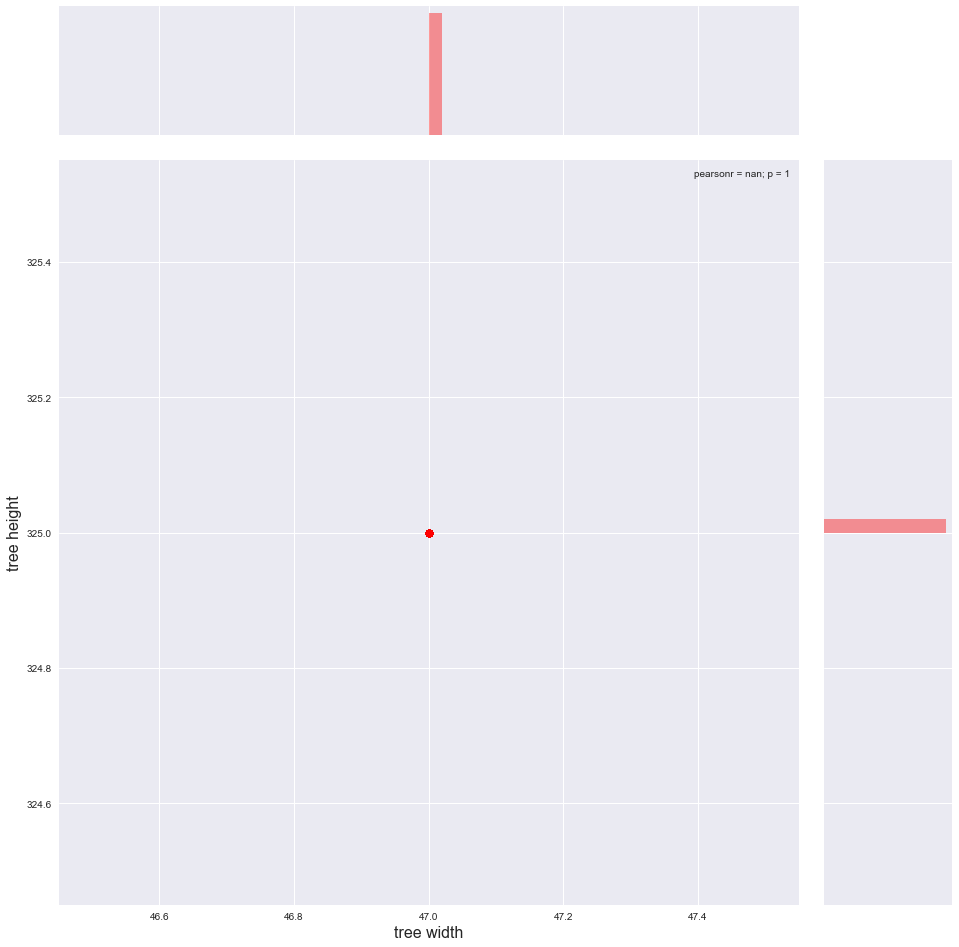
\includegraphics[width=0.5\textwidth]{img/0_UNIFORM_plot.png}
	\caption{Data distribution for 0\_Uniform.in. Source: compiled by the authors.}
	\label{fig:data:uniform}
\end{figure}

\section{Random}
The random data set consists of options with both uniformly distributed random widths and uniformly distributed random heights. This data set is interesting, as it presents a wide variety of options. Both padding and sorting can benefit the processing of such a data distribution, hence the data set can help answer questions concerned with the various optimization techniques that can possibly improve the performance of the algorithm. The random data set we have generated has the following statistics: \\\\
widths: min 7, max 1023, mean 510.77, variance 85197.14, std 291.89, skewness 0.01, kurthosis -1.20.\\\\
heights: min 13, max 1201, mean 605.27, variance 119988.40, std 346.39, skewness 0.01, kurthosis -1.20.

\begin{figure}[H]
	\centering
	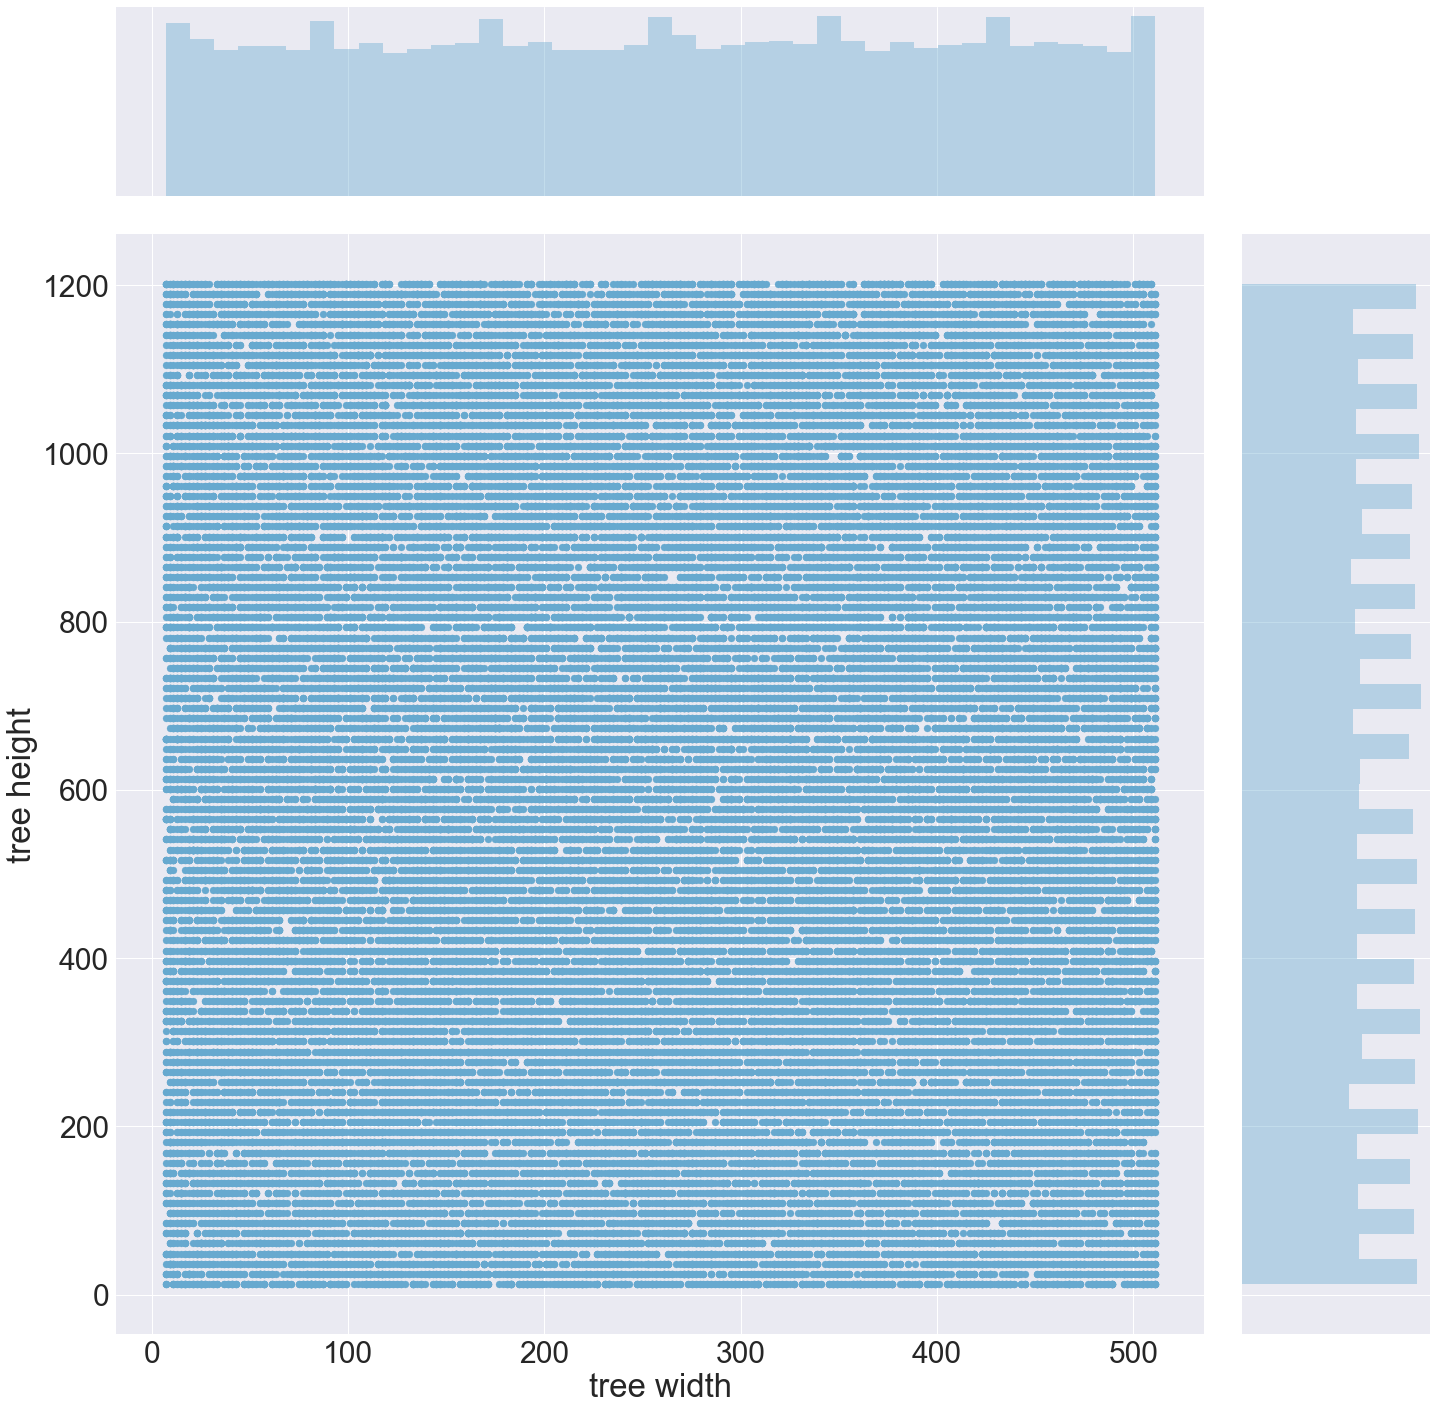
\includegraphics[width=0.5\textwidth]{img/1_RAND_plot.png}
	\caption{Data distribution for 1\_RAND.in. Source: compiled by the authors.}
	\label{fig:data:random}
\end{figure}

\section{Random with constant height/width}
The following two data sets (see fig. \ref{fig:data:randconstheight} and fig. \ref{fig:data:randconstwidth}) have a similar structures to the random one described above, however one of their parameters is being held in place (constant). In the case of constant height, the width is uniformly random distributed, while the height remains the same throughout all options. The other set is vice verse, where the width remains the same, while the height is randomly distributed. These data sets should help strengthen the importance of sorting and padding and the performance improvements they can introduce. The first set - random with constant height consists of 17870 options and deviates by 0.0030964\% from the initial approximation, while the second set - random with constant width consists of 4922 options and deviates by 0.0226458\%. It can be observed that when the height is held constant, the number of options is significantly larger. This occurs, because heights span between 10 and 10000, while widths span between 7 and 1023. Hence, the $width*height$ product increases drastically with options that have large heights. 

\begin{figure}[H]
\centering
\begin{subfigure}{.5\textwidth}
  \centering
  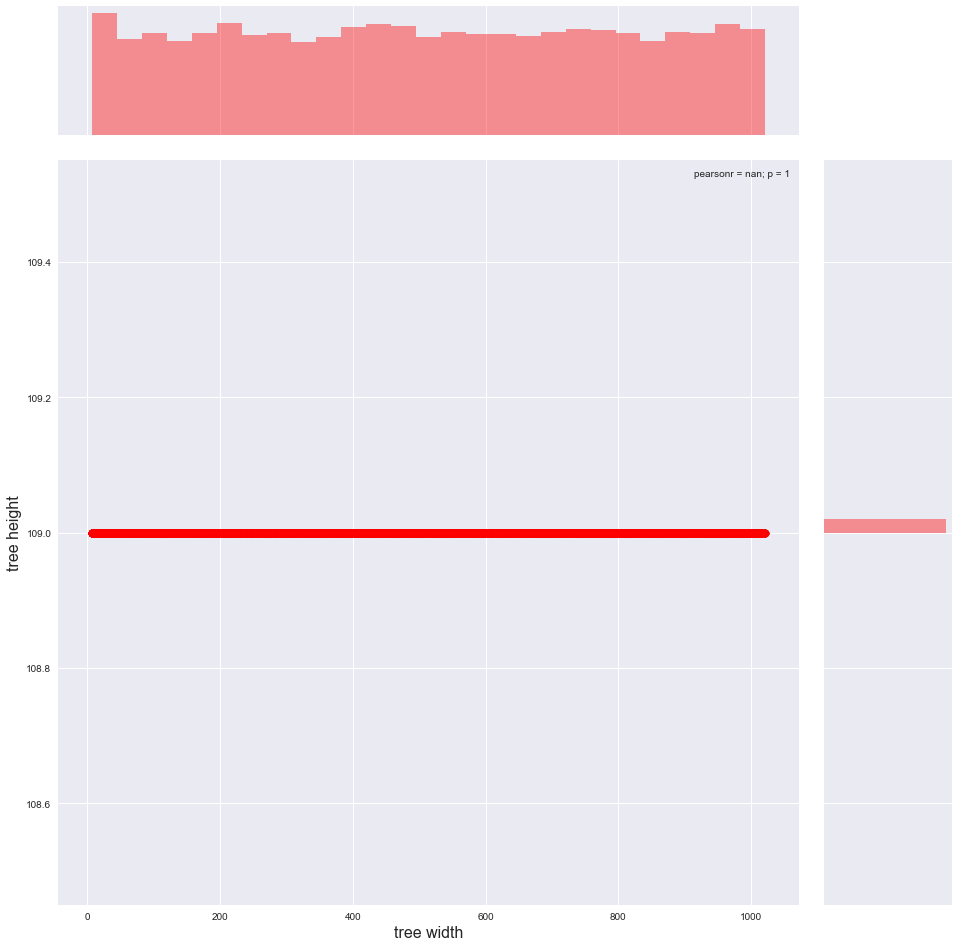
\includegraphics[width=.8\linewidth]{img/2_RANDCONSTHEIGHT_plot.png}
  \caption{Constant height}
  \label{fig:data:randconstheight}
\end{subfigure}%
\begin{subfigure}{.5\textwidth}
  \centering
  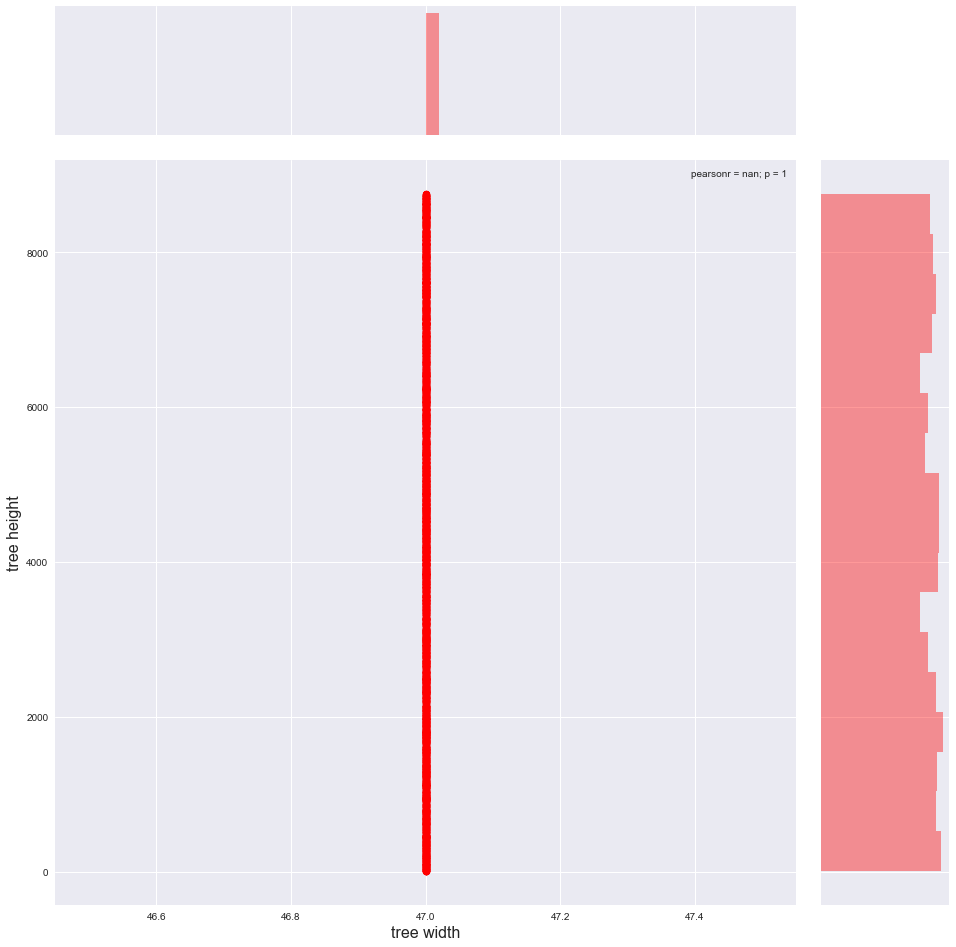
\includegraphics[width=.8\linewidth]{img/3_RANDCONSTWIDTH_plot.png}
  \caption{Constant width}
  \label{fig:data:randconstwidth}
\end{subfigure}
\caption{Data distributions for 2\_RANDCONSTHEIGHT.in (a) and 3\_RANDCONSTWIDTH.in. Source: compiled by the authors.}
\label{fig:test}
\end{figure}

\section{Skewed}
This data set introduces data skewness, where a small percent of all options is significantly different than the rest. As it can be seen in fig. \ref{fig:data:skewed} the majority of the data has widths up to 450 and heights up to 100. Standing out are several options with much larger heights and widths. This data distribution can also often occur in real life situations, where several data entries significantly deviate from the rest. This introduces problems with memory padding in some of the implementations, but it can benefit from sorting both along the height and along the width. It is further interesting to observe whether cuda-multi can produce any performance increase on data sets where the majority of options have small widths, hence allowing to pack and process several options in parallel. The data set we have generated with this distribution consists of 8554 options, 8 of which (5\%) significantly different, with a total $width*height$ sum of 1000215596, deviating from the initial approximation by 0.0215596\%.

\begin{figure}[H]
	\centering
	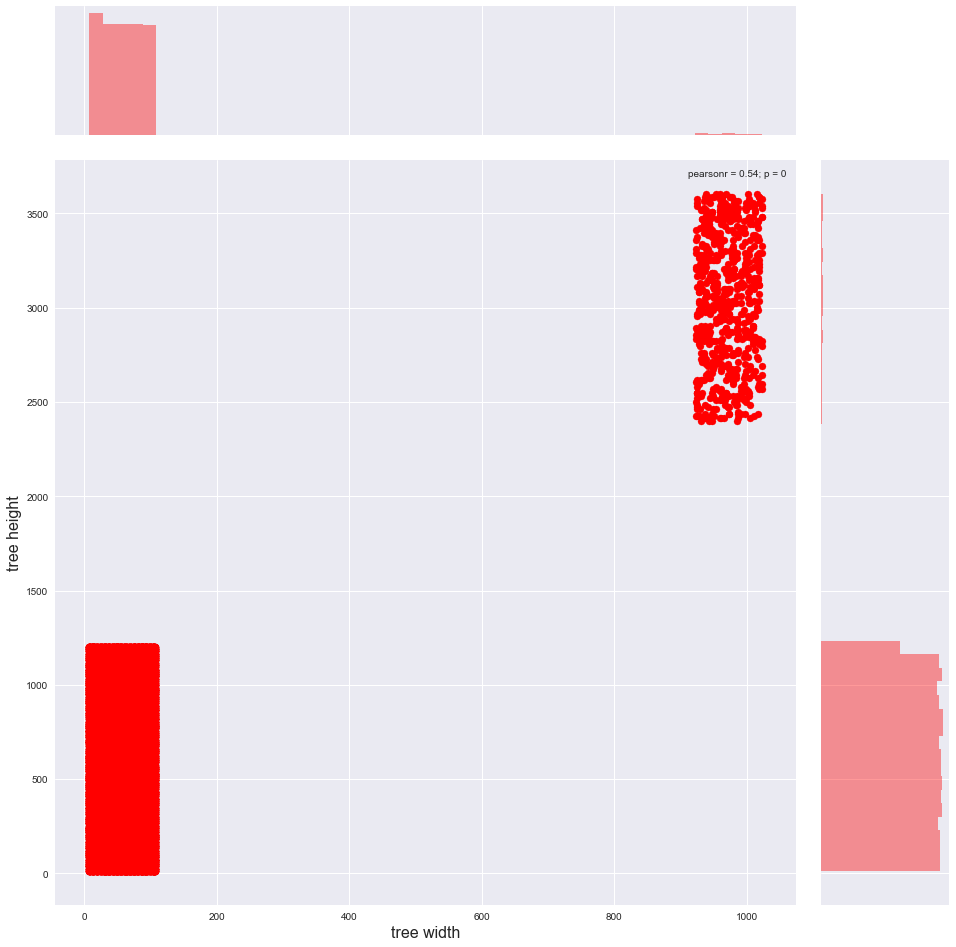
\includegraphics[width=0.5\textwidth]{img/4_SKEWED_plot.png}
	\caption{Data distribution for 4\_SKEWED.in. Source: compiled by the authors.}
	\label{fig:data:skewed}
\end{figure}

\section{Skewed with constant height/width}
The last two data sets (see fig. \ref{fig:data:skewedconstheight} and fig. \ref{fig:data:skewedconstwidth}) introduce similar concepts as the random constant height/width data sets. Here the majority of the data has a uniform random distribution on both axes, however one of the axes creates a limit - max value. E.g. in the skewed with constant height data set, the width is limited to 450, while the height can take any number in the range 10 to 10000. The skewed part of this data set has a constant height, which does not stand out from the other options, differently from the width, which varies in a much larger spectrum. This is also done vice verse on the other set - skewed with constant width, which the majority of options consists of options with varying width, but low heights and a skewed part, consisting of a small fixed width and heights within a larger spectrum. The purpose of these sets is to put emphasis on the impact that large widths and large heights can have on the implementations and strengthen the performance increase hypotheses when sorting and padding is performed.

\begin{figure}[H]
\centering
\begin{subfigure}{.5\textwidth}
  \centering
  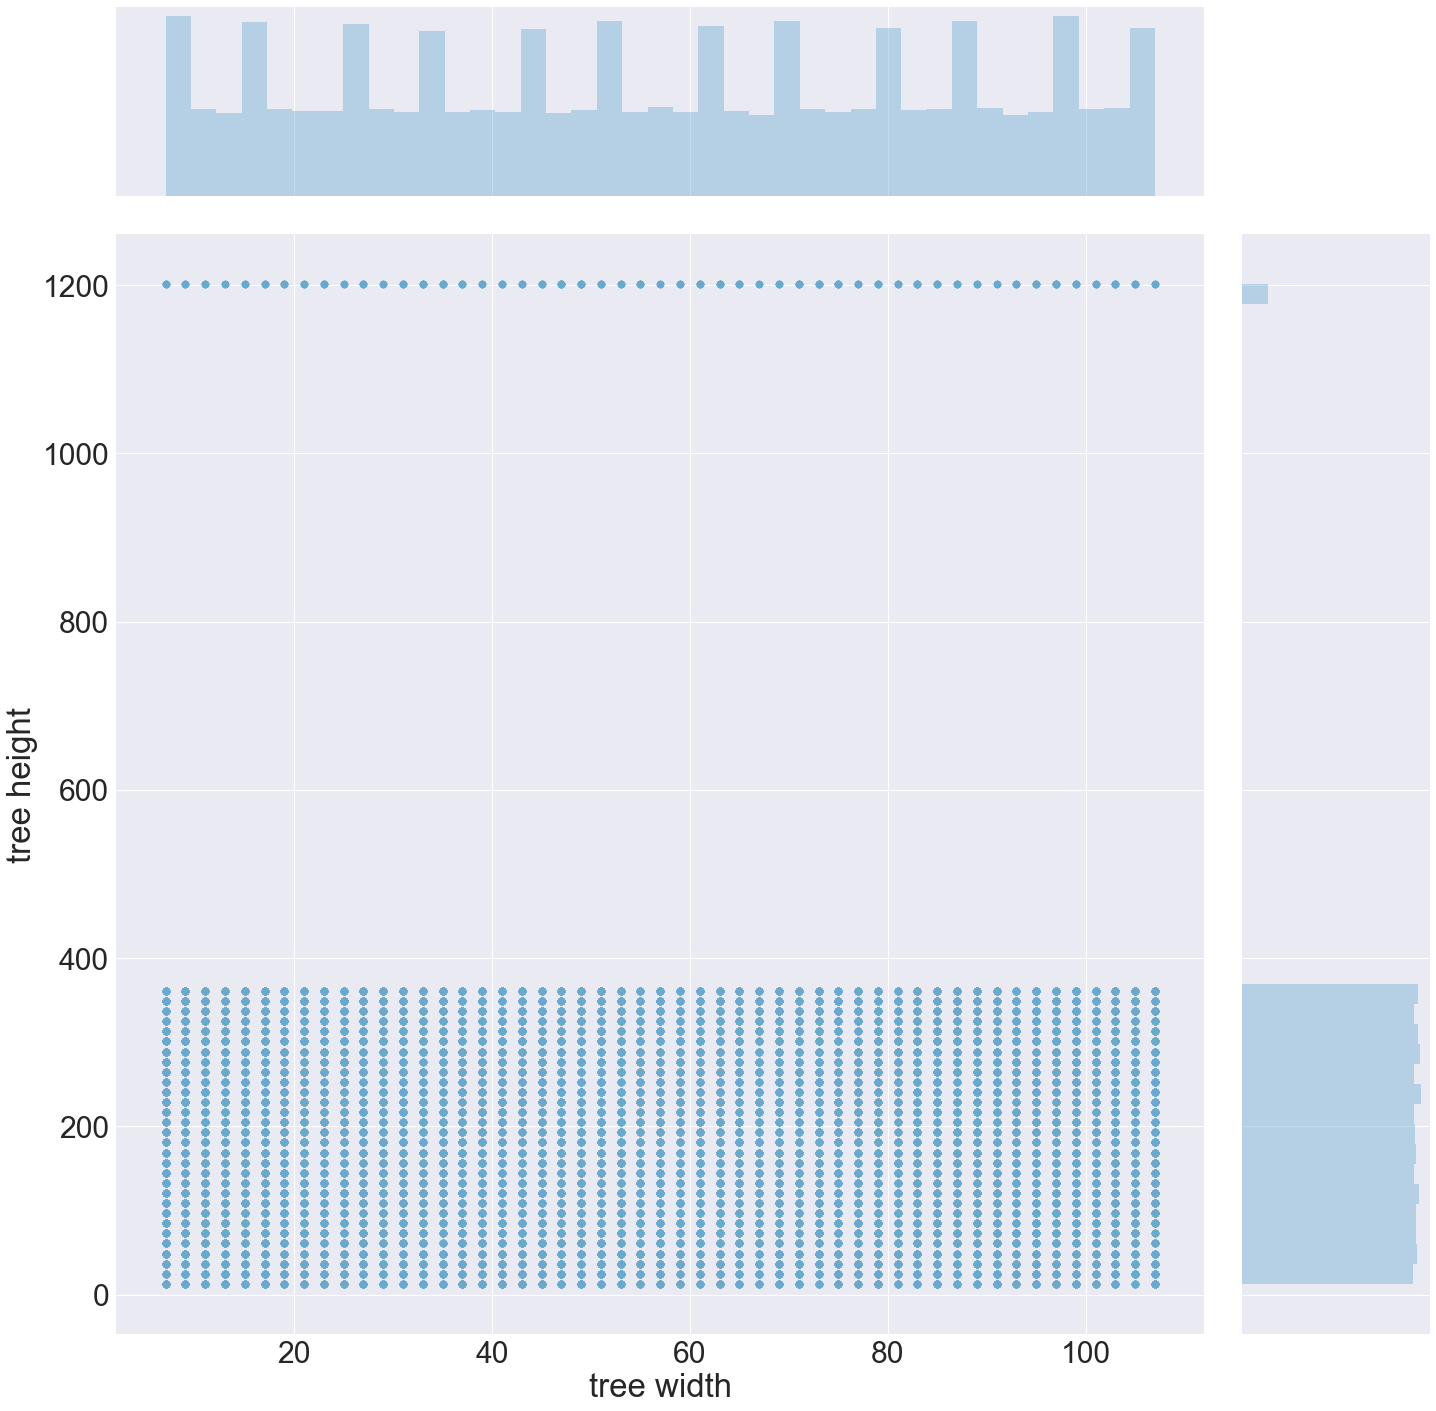
\includegraphics[width=.8\linewidth]{img/5_SKEWEDCONSTHEIGHT_plot.png}
  \caption{Constant height}
  \label{fig:data:skewedconstheight}
\end{subfigure}%
\begin{subfigure}{.5\textwidth}
  \centering
  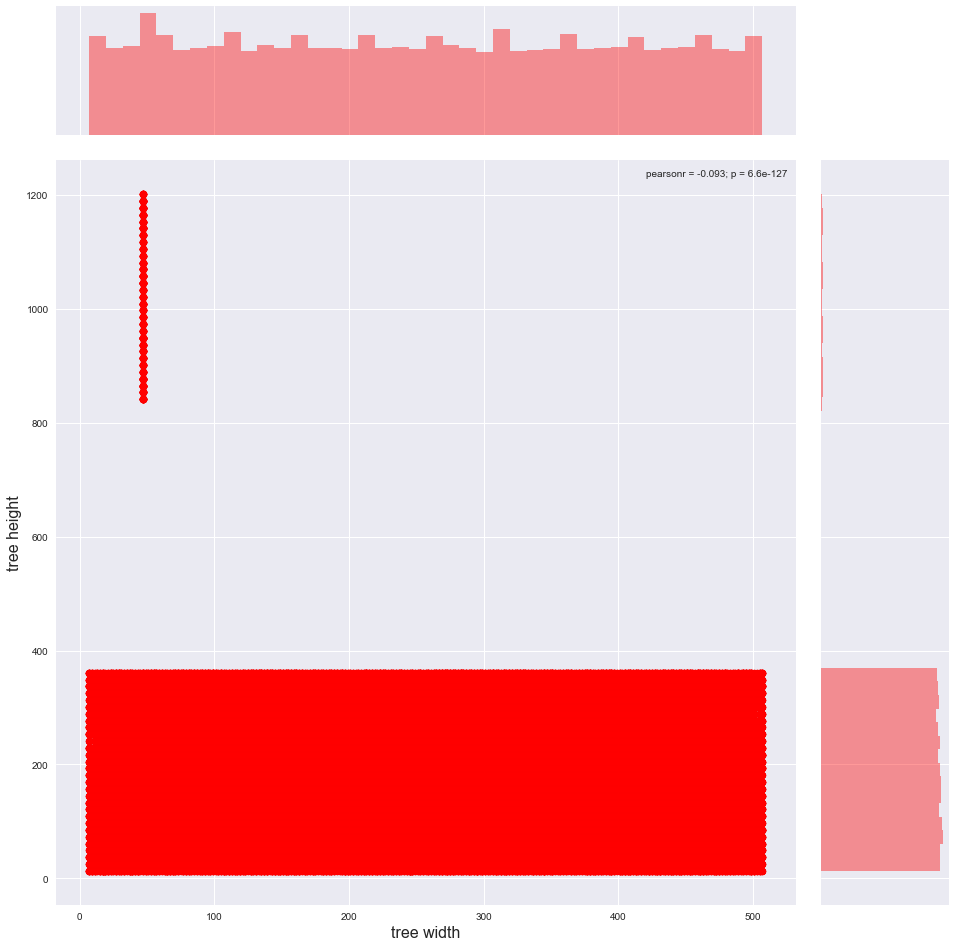
\includegraphics[width=.8\linewidth]{img/6_SKEWEDCONSTWIDTH_plot.png}
  \caption{Constant width}
  \label{fig:data:skewedconstwidth}
\end{subfigure}
\caption{Data distributions for 5\_SKEWEDCONSTHEIGHT.in (a) and 6\_SKEWEDCONSTWIDTH.in. Source: compiled by the authors.}
\label{fig:test}
\end{figure}

% \section{Other data used}
% - a bit about Wojciechs data maybe ?

\section*{Summary}
This chapter has introduced the reader to the different data sets that have been generated to support the thesis. While not all of them seem realistic in practise, their purpose is to cover edge cases, which can occur seldomly in real-life scenarios. Using these sets can help discover not possible bugs in the implementations, when working with different data, as well as highlight on the performance between the versions and parallelism used to process data. Last, but not least, as mentioned several times throughout the chapter, many of the data sets can be used to discover the advantages and disadvantages of optimization techniques, such as sorting and memory padding. The data sets will be used in order to obtain running times and create benchmarks for the algorithm and the different implementations with their versions. Benchmarking will be described in the next chapter - \ref{chapter:benchmarking}.